\documentclass{beamer}
\usetheme{Warsaw}
\setbeamertemplate{headline}{}

\usepackage{ae,lmodern}
\usepackage[english]{babel}
\usepackage[utf8]{inputenc}
\usepackage[T1]{fontenc}

\usepackage{caption}
\captionsetup[figure]{labelformat=empty}

\PassOptionsToPackage{usenames,dvipsnames}{xcolor}
\usepackage{xcolor,colortbl}
\definecolor{DarkGrey}{HTML}{222222}
\definecolor{DarkBlue}{HTML}{004BA9}
\definecolor{DarkRed}{HTML}{CC1111}
\definecolor{DarkGreen}{HTML}{117711}
\definecolor{DarkOrange}{HTML}{CC7000}
\definecolor{LightGrey}{HTML}{DDDDDD}
\definecolor{LightBlue}{HTML}{F0F8FF}
\definecolor{codegreen}{rgb}{0,0.6,0}
\definecolor{codepurple}{rgb}{0.58,0,0.82}

\usepackage[cache=false]{minted}
\setminted[bash]{
   bgcolor=LightBlue,
   breaklines, breakanywhere,
   frame=single,
   autogobble
}
\usemintedstyle[python]{native}
\setminted[python]{
   bgcolor=black,
   breaklines, breakanywhere,
   autogobble
}

\usepackage{listings}
\usepackage{lstautogobble}
\lstdefinestyle{bash}{
    backgroundcolor=\color{DarkGrey},   
    commentstyle=\color{codegreen},
    keywordstyle=\color{magenta},
    numberstyle=\tiny\color{DarkGrey},
    stringstyle=\color{codepurple},
    basicstyle=\ttfamily\tiny\color{LightGrey},
    escapeinside={\%*}{*)},
    breakatwhitespace=false,         
    breaklines=true,                 
    captionpos=b,                    
    keepspaces=true,                 
    numbers=left,                    
    numbersep=5pt,                  
    showspaces=false,                
    showstringspaces=false,
    showtabs=false,
    showlines=false,
    tabsize=2
}

\usepackage{tikz}
\usetikzlibrary{calc,decorations.pathreplacing,arrows,arrows.meta,shapes,patterns, positioning}
\newcommand\BigLength{14.6em}
\newcommand\Height{2em}
\newcommand\Sep{0.6em}
\newcommand\Center{\BigLength*1/2}
\newcommand\BigBox{\BigLength+\Sep}
\newcommand\HalfBox{\BigLength*1/2-\Sep*1/4}
\newcommand\HalfLength{\BigLength*1/2-\Sep*5/4}
\newcommand\CenterL{\BigLength*1/4-\Sep*1/8}
\newcommand\CenterR{\BigLength*3/4+\Sep*1/8}
\tikzstyle{layer}=[rectangle,thick,text centered,
                     minimum height=\Height,minimum width=\BigLength]
\tikzstyle{short}=[rectangle,thick,text centered,
                     minimum height=\Height,minimum width=\HalfLength]
\tikzstyle{dibox}=[rectangle,thick,semitransparent,
                     minimum height=(\Height+\Sep)*2,minimum width=\BigBox]
\tikzstyle{vmbox}=[rectangle,thick,semitransparent,
                     minimum height=(\Height+\Sep)*3,minimum width=\HalfBox]
\tikzstyle{ctbox}=[rectangle,thick,semitransparent,
                     minimum height=(\Height+\Sep)*2,minimum width=\HalfBox]
\tikzstyle{vebox}=[rectangle,thick,semitransparent,
                     minimum height=(\Height+\Sep)*1,minimum width=\HalfBox]

\usepackage{hyperref}
\usepackage{grffile}


\AtBeginSection[]
{
   \begin{frame}
      \tableofcontents[currentsection]
   \end{frame}
}

\AtBeginSubsection[]
{
   \begin{frame}
      \tableofcontents[currentsection, currentsubsection, sectionstyle=shaded]
   \end{frame}
}

%----------------------------------------------------------------------------------------
\title{Introduction to Data Science}
\subtitle{with Python}
%----------------------------------------------------------------------------------------
\author{Alexis Bogroff}
\date{\today}



\newlength\myheight
\newlength\mydepth
\settototalheight\myheight{Xygp}
\settodepth\mydepth{Xygp}
\setlength\fboxsep{0pt}
\newcommand*\inlinegraphics[1]{%
  \settototalheight\myheight{Xygp}%
  \settodepth\mydepth{Xygp}%
  \raisebox{-\mydepth}{\includegraphics[height=\myheight]{#1}}%
}

\begin{document}


\begin{frame}
   \titlepage
\end{frame}

\begin{frame}\frametitle{Presenter}
   \begin{minipage}{0.3\linewidth}
      \centering
      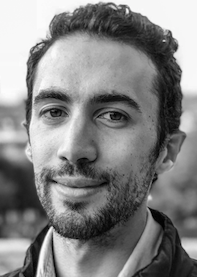
\includegraphics[width=0.6\textwidth]{../images/AlexisBogroff.png} \\
   \end{minipage}
   \begin{minipage}{0.6\linewidth}
      \noindent Alexis Bogroff \\
      Lecturer and Mentor in Data Science \\
      at Paris 1 Panthéon-Sorbonne, ESILV, Openclassrooms, EM-Lyon
   \end{minipage}
   \\[2ex]
   \visible<2->{\begin{itemize}
      \item 4 years Teaching Assistant and lecturer in VBA, Python for finance, SQL, Data Analysis and Data Science
      \item 9 months Researcher Assistant at Paris 1 Panthéon-Sorbonne within H2020 European Project
      \item 1 year Data Scientist at Pléiade Asset Management
   \end{itemize}}
   \hfill
\end{frame}

% \begin{frame}\frametitle{Overview}
%    \Large
%    \centering
%    Financial Engineering with Python Linux and Git \\[2ex]
%    \begin{minipage}{0.32\linewidth}
%       \includegraphics[width=0.8\textwidth]{../images/linux-1-logo-svg-vector.pdf}
%    \end{minipage}
%    \begin{minipage}{0.32\linewidth}
%       \includegraphics[width=0.8\textwidth]{../images/Git-logo.pdf}
%    \end{minipage}
%    \begin{minipage}{0.32\linewidth}
%       \includegraphics[width=0.9\textwidth]{../images/Python_logo_and_wordmark.pdf}
%    \end{minipage}
%    \pause
%    \\[3ex]
%    Free and everywhere stack \\
%    To find a job and be operational
% \end{frame}

% \begin{frame}\frametitle{Lecture Organisation}
%    \begin{itemize}[<+->]
%       \item Prerequisite:
%       \begin{enumerate}
%          \item Have a Linux environment working on your personal computer
%          \item[] (it can be WSL2 on Windows, Amazon EC2 for a distant solution)
%          \item Install Git
%          \item Install Python
%       \end{enumerate}
%       \vspace{2em}
%       \item Exam:
%       \begin{itemize}
%          \item Last QCM 1/2
%          \item Project 1/2
%       \end{itemize}
%    \end{itemize}
% \end{frame}


\begin{frame}
   \tableofcontents
\end{frame}

% =============================================================================
% =============================================================================
\section{Overview}
% 3 Hours course
% =============================================================================
% =============================================================================


%------------------------------------------------------------------------------
\subsection{Why this course}
%------------------------------------------------------------------------------
\begin{frame}\frametitle{Why this course}
   \begin{itemize}
      % \item TODO: find article about current enormous investments made to collect and work on data, data analysts, data scientist
      % \item TODO: find article about jobs using data even though they are not data scientists
      % \item TODO: find graphs about these points
      \item You already work in a data rich environment
      \item Benefit from upskilling in Data Science \inlinegraphics{../images/illustrations/up_arrow_green.png}
   \end{itemize}


   \begin{figure}[H]
      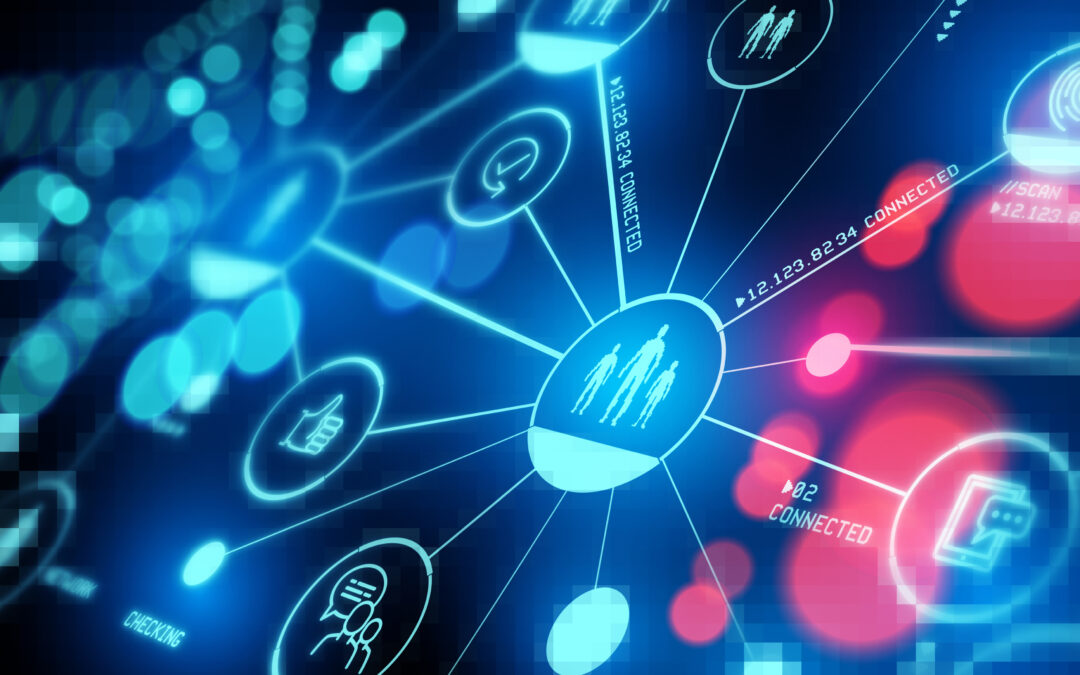
\includegraphics[width=10cm]{../images/illustrations/data_everywhere.jpeg}
   \end{figure}
\end{frame} 

\begin{frame}\frametitle{Why this course}
   \begin{itemize}
      \item Short 3 days course \inlinegraphics{../images/illustrations/run.jpeg}
      \item Objective 1: understand the current data ecosystem
      \begin{itemize}
         \item Fundamental components
         \item Their (intricated) links
      \end{itemize}
      \begin{figure}[H]
         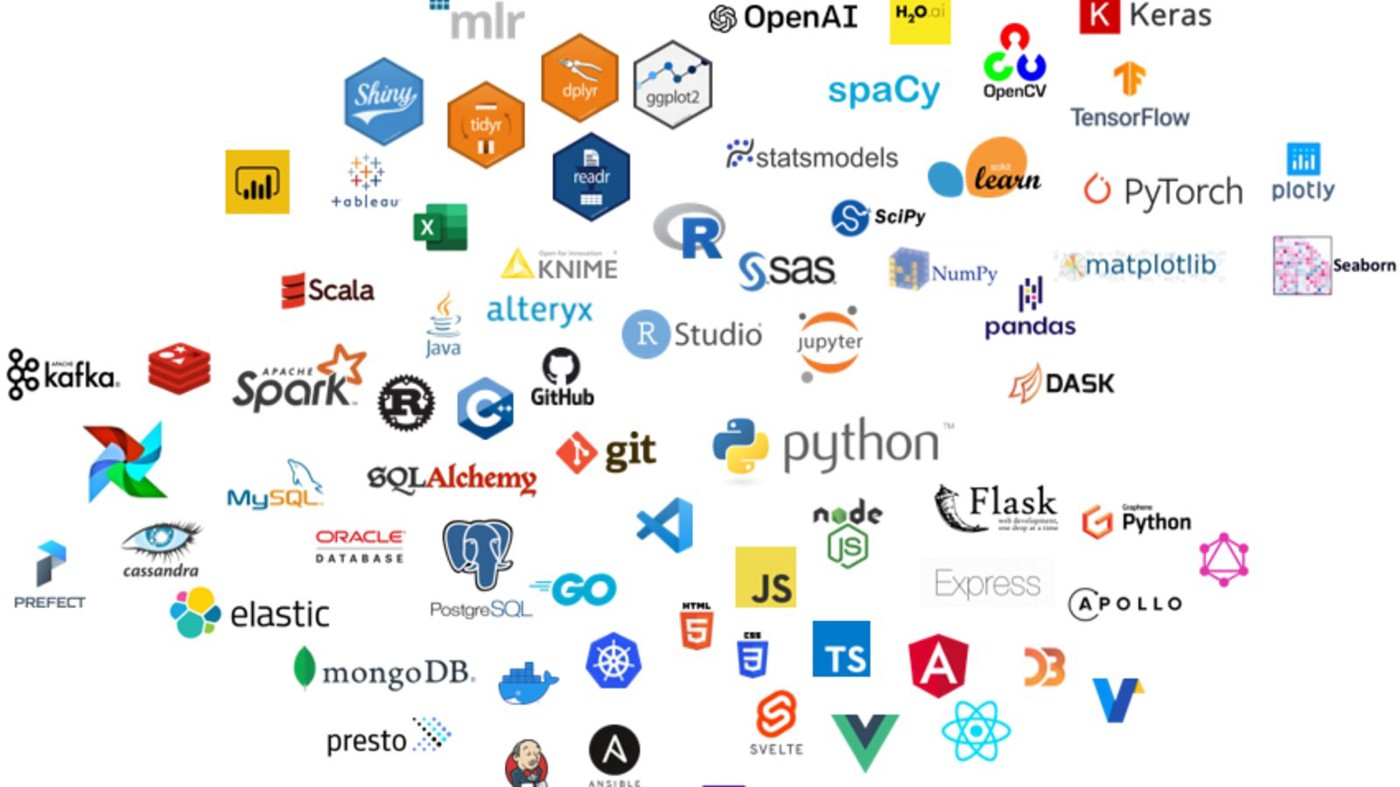
\includegraphics[width=10cm]{../images/illustrations/data_ecosystem.png}
      \end{figure}
   \end{itemize}
\end{frame}


\begin{frame}\frametitle{Why this course}
   \begin{itemize}
      \item Objective 2: confidence in your abilities to learn by yourself
      \begin{itemize}
         \item Understand theoretical points
         \item Practice
      \end{itemize}
      \item Comparison to complete formations (3 days vs 1 year)
   \end{itemize}

   \begin{figure}[H]
      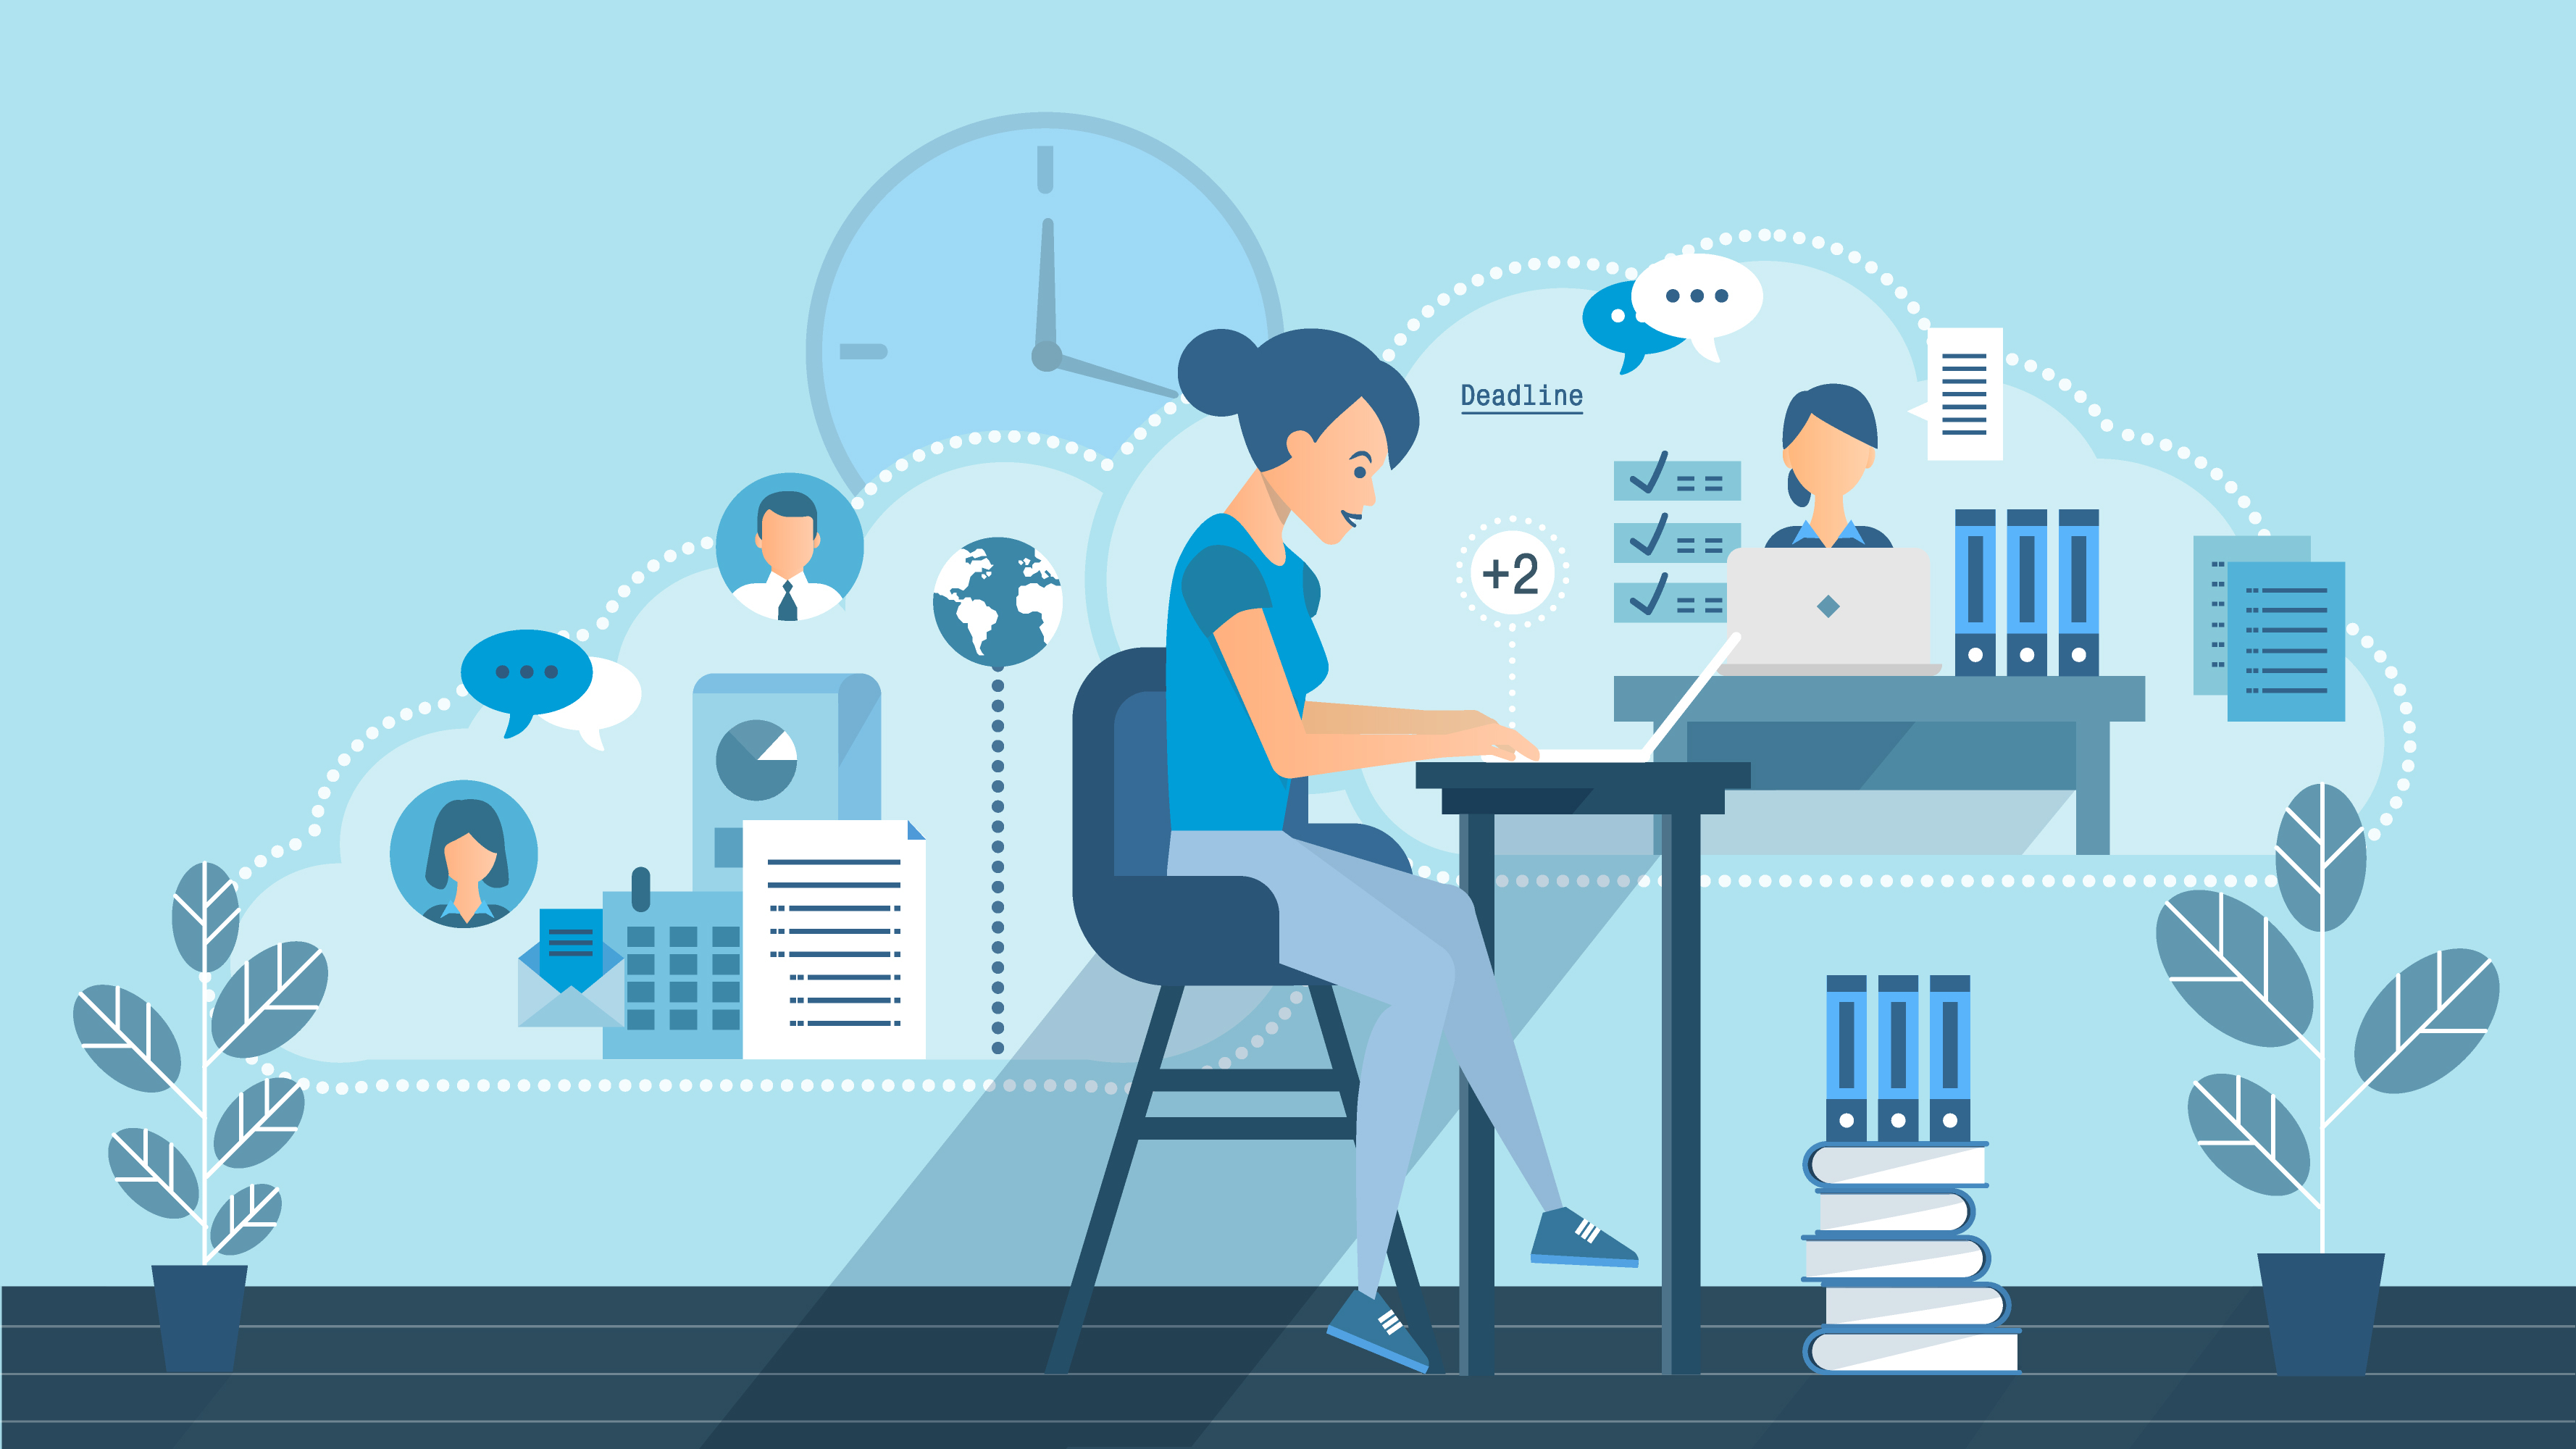
\includegraphics[width=10cm]{../images/illustrations/learn_autonomous.jpeg}
   \end{figure}

\end{frame}


%------------------------------------------------------------------------------
\subsection{What is Artificial Intelligence}
%------------------------------------------------------------------------------
% Explanation of main Key Words: Deep Learning
% And Current Trends
\begin{frame}\frametitle{What is Artificial Intelligence}
   \begin{itemize}
      \item Artificial Intelligence = Marketing
      \item Machine Learning (ML) = Technical
   \end{itemize}
   \vspace*{20px}
   \begin{minipage}{0.48\linewidth}
      \begin{figure}[H]
         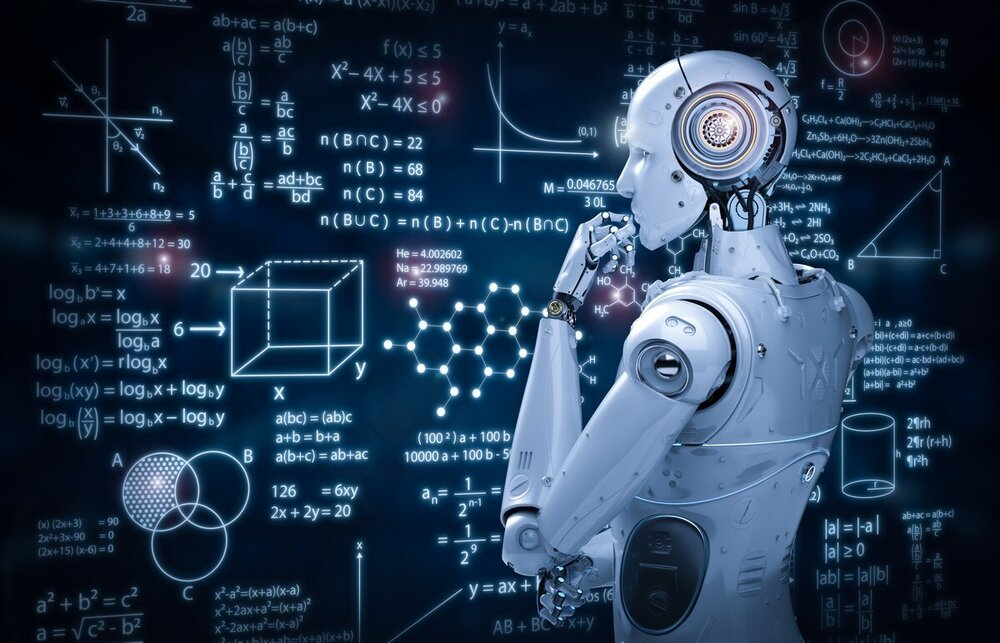
\includegraphics[width=6cm]{../images/illustrations/ai.jpeg}
      \end{figure}
   \end{minipage}
   \begin{minipage}{0.48\linewidth}
      \begin{figure}[H]
         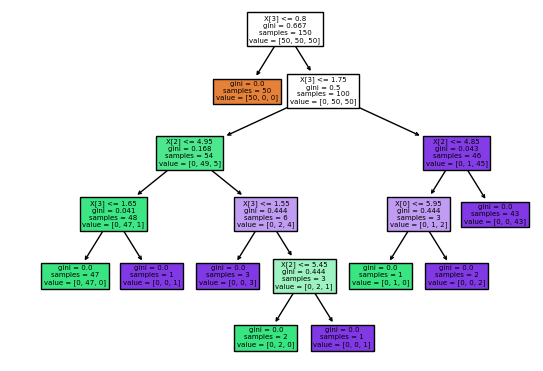
\includegraphics[width=6cm]{../images/illustrations/tree.png}
      \end{figure}
   \end{minipage}
\end{frame}

\begin{frame}\frametitle{What is Artificial Intelligence}
   \begin{itemize}
      \item New word for old models
      \item Simple models answer to most business problems
      \item Automation and rules (programming, manual analysis) often required
      \item Machine learning often overkill
      \item ML requires a lot of \textbf{clean} data
      \footnote{\href{https://landing.ai/data-centric-ai/}{https://landing.ai/data-centric-ai/}}
   \end{itemize}
   \vspace*{20px}
   \begin{minipage}{0.48\linewidth}
      \begin{figure}[H]
         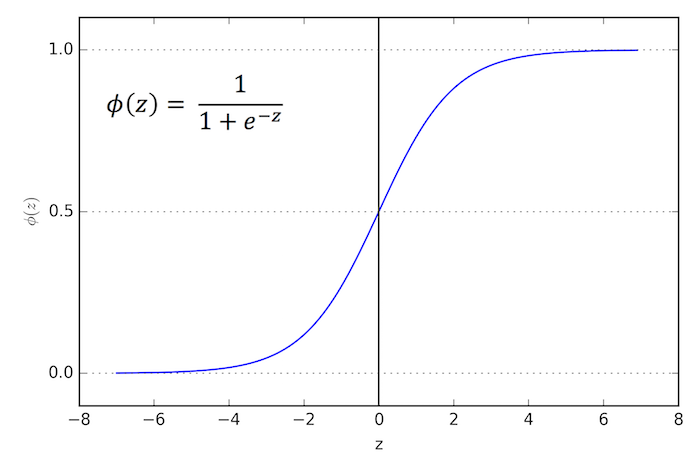
\includegraphics[width=4cm]{../images/illustrations/logistic.png}
      \end{figure}
   \end{minipage}
   \begin{minipage}{0.48\linewidth}
      \begin{figure}[H]
         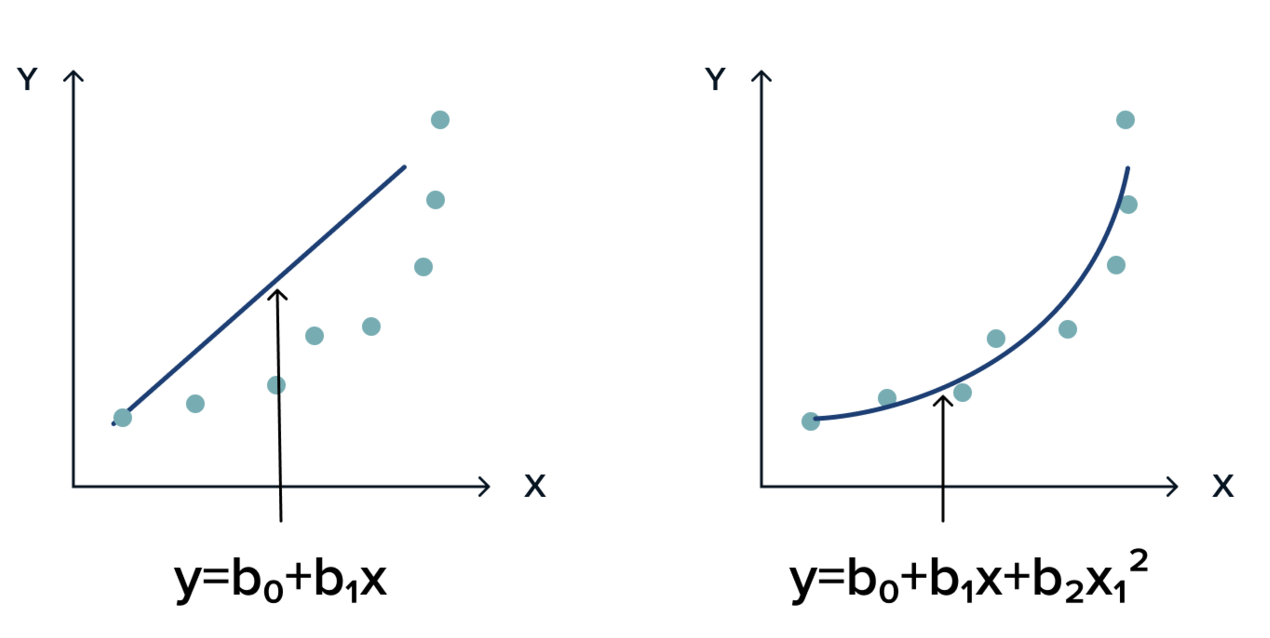
\includegraphics[width=6cm]{../images/illustrations/polynomial.png}
      \end{figure}
   \end{minipage}
\end{frame}

\begin{frame}\frametitle{Where is Machine Learning (almost) necessary?}
   \begin{itemize}      
      \item State Of The Art (SOTA) Deep Learning models:
      \begin{itemize}
         \item Computer vision: e.g. object detection, face recognition, etc.)
         \item Autonomous driving (but Lidar...)
         \item Recommander systems
         \item Natural Language Processing (NLP) e.g. Translation
      \end{itemize}
   \end{itemize}
   \begin{minipage}{0.48\linewidth}
      \begin{figure}[H]
         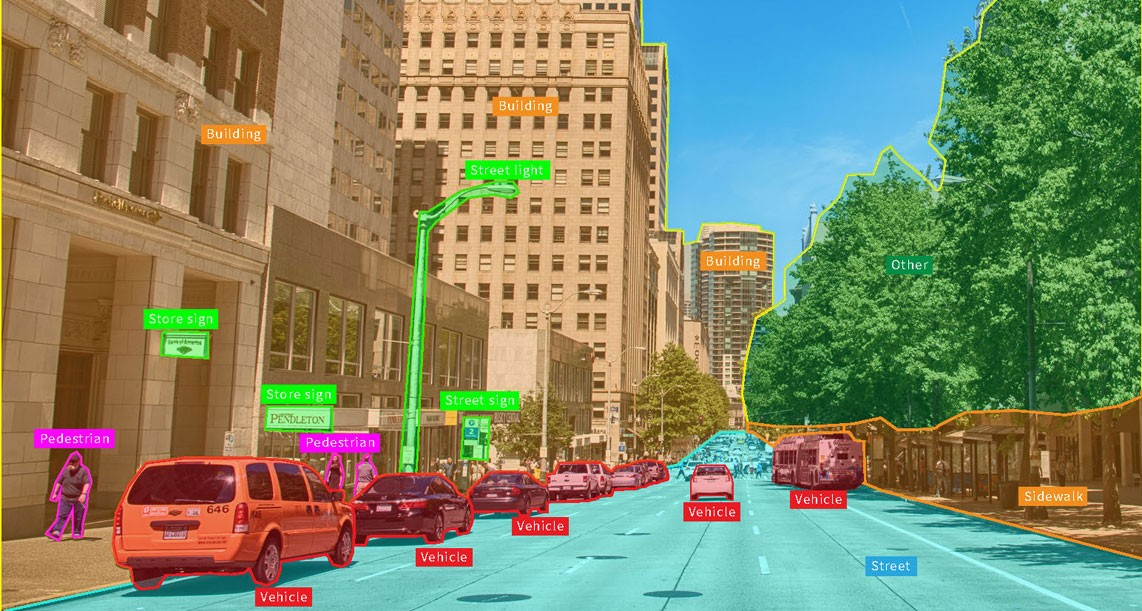
\includegraphics[width=4cm]{../images/illustrations/objects-detection.jpeg}
      \end{figure}
   \end{minipage}
   \begin{minipage}{0.48\linewidth}
      \begin{figure}[H]
         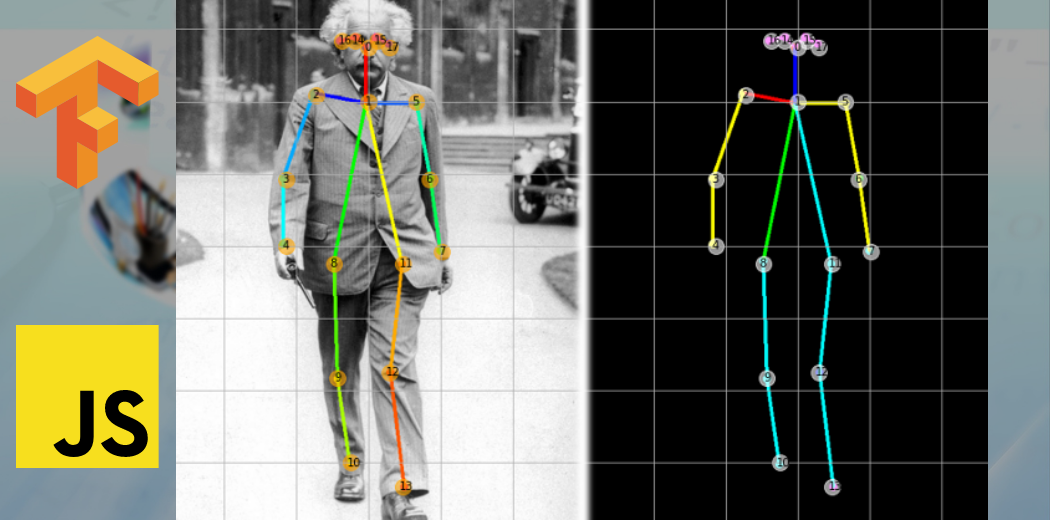
\includegraphics[width=4cm]{../images/illustrations/posenet.png}
      \end{figure}
   \end{minipage}

   \begin{minipage}{0.48\linewidth}
      \begin{figure}[H]
         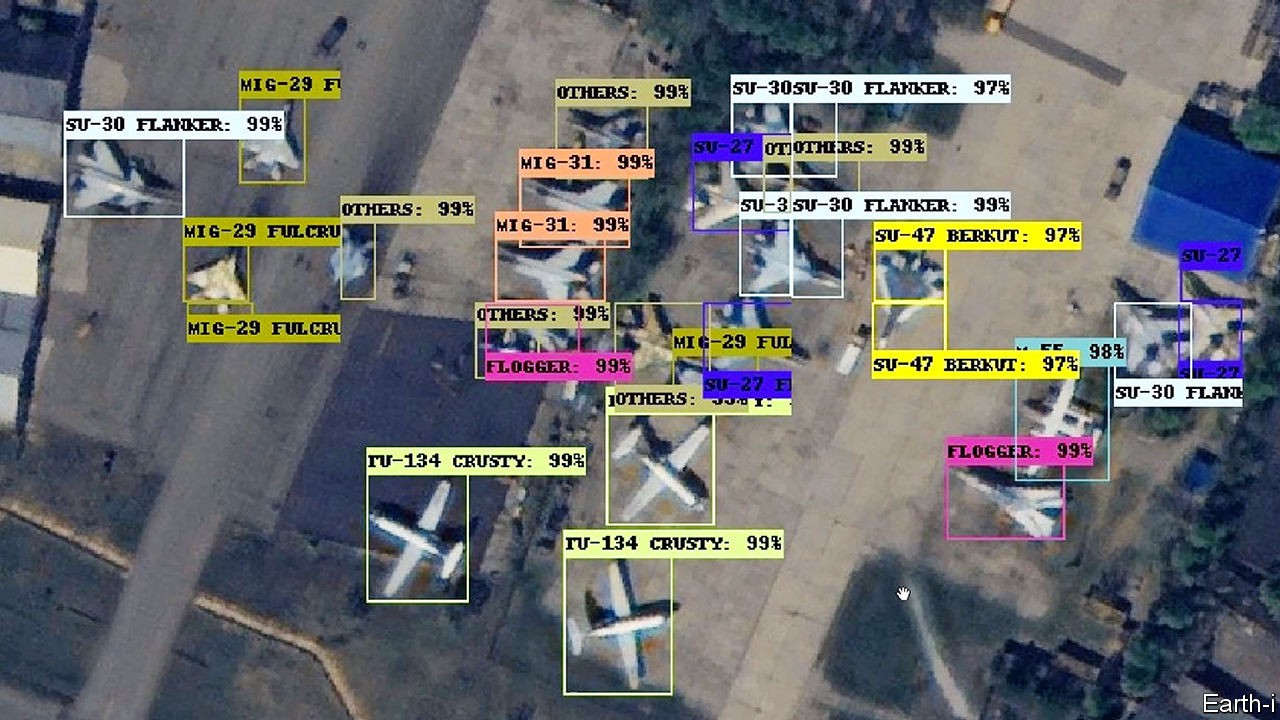
\includegraphics[width=4cm]{../images/illustrations/satellite.jpeg}
      \end{figure}
   \end{minipage}
   \begin{minipage}{0.48\linewidth}
      \begin{figure}[H]
         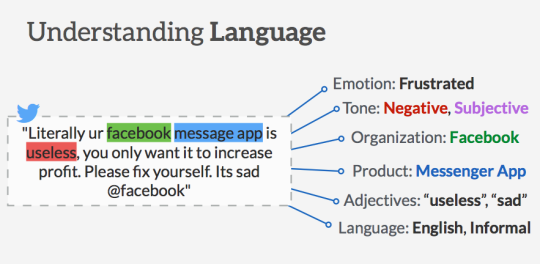
\includegraphics[width=6cm]{../images/illustrations/nlp.png}
      \end{figure}
   \end{minipage}

   \begin{minipage}{0.2\linewidth}
      \begin{figure}[H]
         
\includegraphics[width=1.5cm]{../images/illustrations/netflix.jpeg}
      \end{figure}
   \end{minipage}
   \begin{minipage}{0.1\linewidth}
      \begin{figure}[H]
         
\includegraphics[width=0.8cm]{../images/illustrations/spotify.jpeg}
      \end{figure}
   \end{minipage}
   \begin{minipage}{0.1\linewidth}
      \begin{figure}[H]
         
\includegraphics[width=2cm]{../images/illustrations/amazon.png}
      \end{figure}
   \end{minipage}

\end{frame}


\begin{frame}\frametitle{Use cases}
   \begin{itemize}
      \item At your reach:
      \vspace*{20px}
      \begin{itemize}
         \item Fraud detection
         \begin{minipage}{0.1\linewidth}
            \begin{figure}[H]
               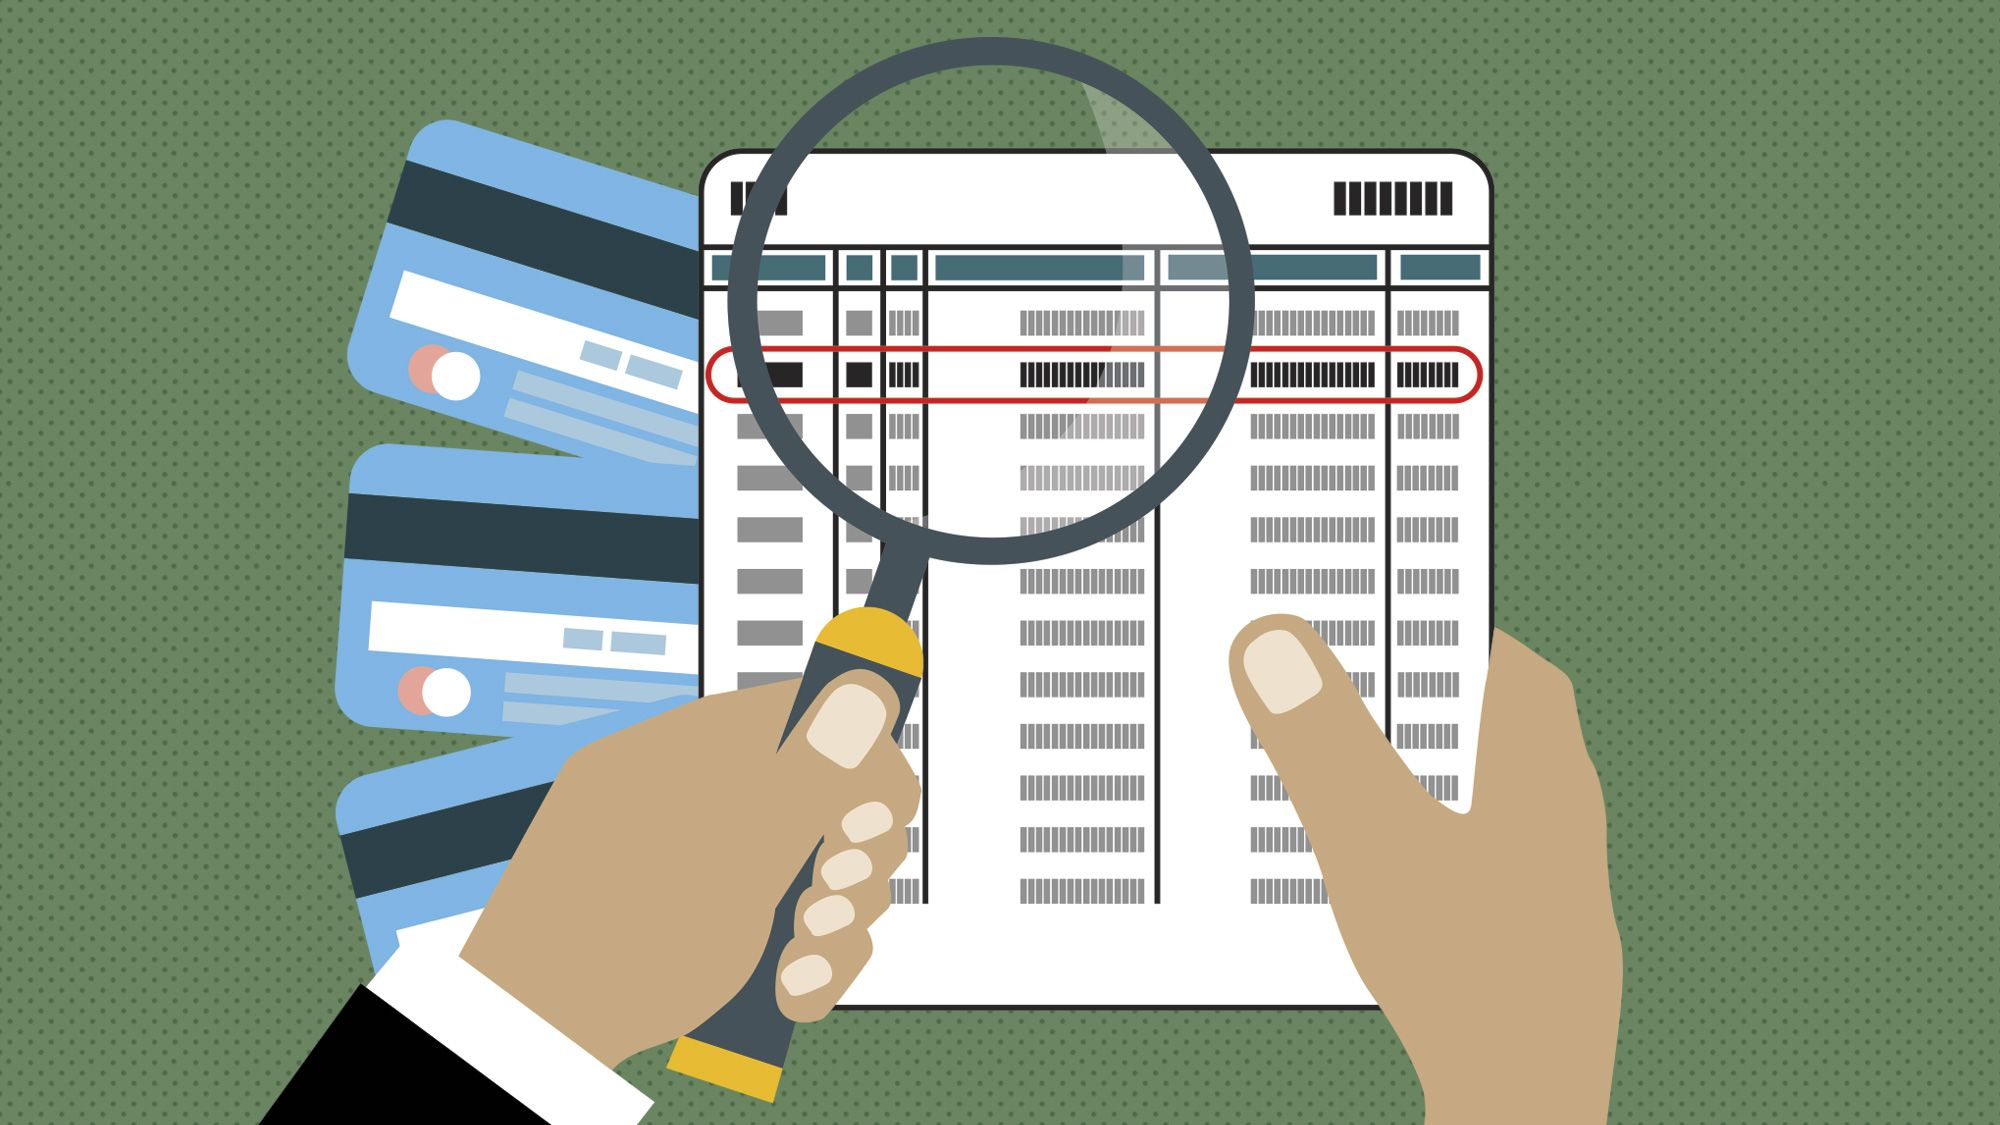
\includegraphics[width=2cm]{../images/illustrations/fraud.jpeg}
            \end{figure}
         \end{minipage}
         \item Client segmentation
         \begin{minipage}{0.1\linewidth}
            \begin{figure}[H]
               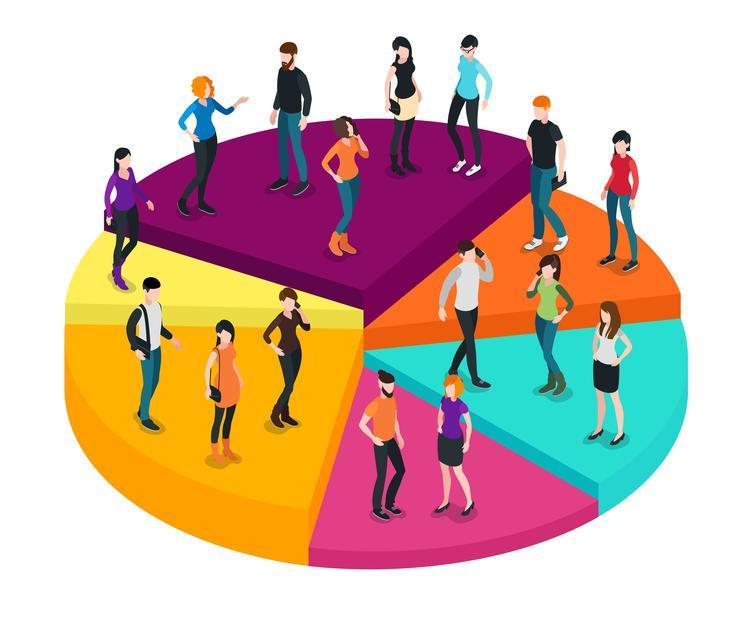
\includegraphics[width=2cm]{../images/illustrations/client_segmentation.jpeg}
            \end{figure}
         \end{minipage}
         \item Revenue, expenditures, commands prediction
         \begin{minipage}{0.1\linewidth}
            \begin{figure}[H]
               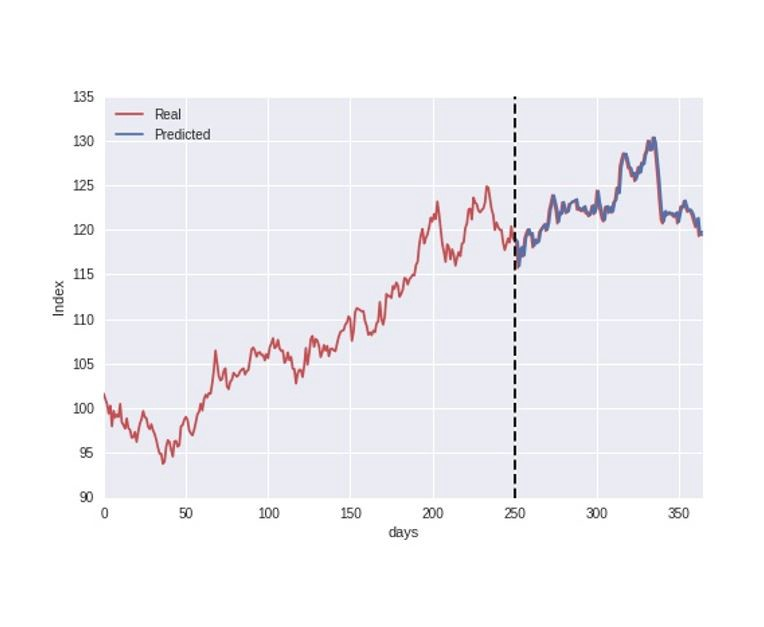
\includegraphics[width=3cm]{../images/illustrations/time_series_pred.jpeg}
            \end{figure}
         \end{minipage}
      \end{itemize}
   \end{itemize}
\end{frame}


\begin{frame}\frametitle{Use cases}
   \begin{itemize}
      \item Not yet for you:
      \begin{itemize}
         \item (Good) Chatbots
         \begin{minipage}{0.2\linewidth}
            \begin{figure}[H]
               
\includegraphics[width=4cm]{../images/illustrations/chatbot.png}
            \end{figure}
         \end{minipage}
         
         \item Sattelite imagery based predictions
         \begin{minipage}{0.2\linewidth}
            \begin{figure}[H]
               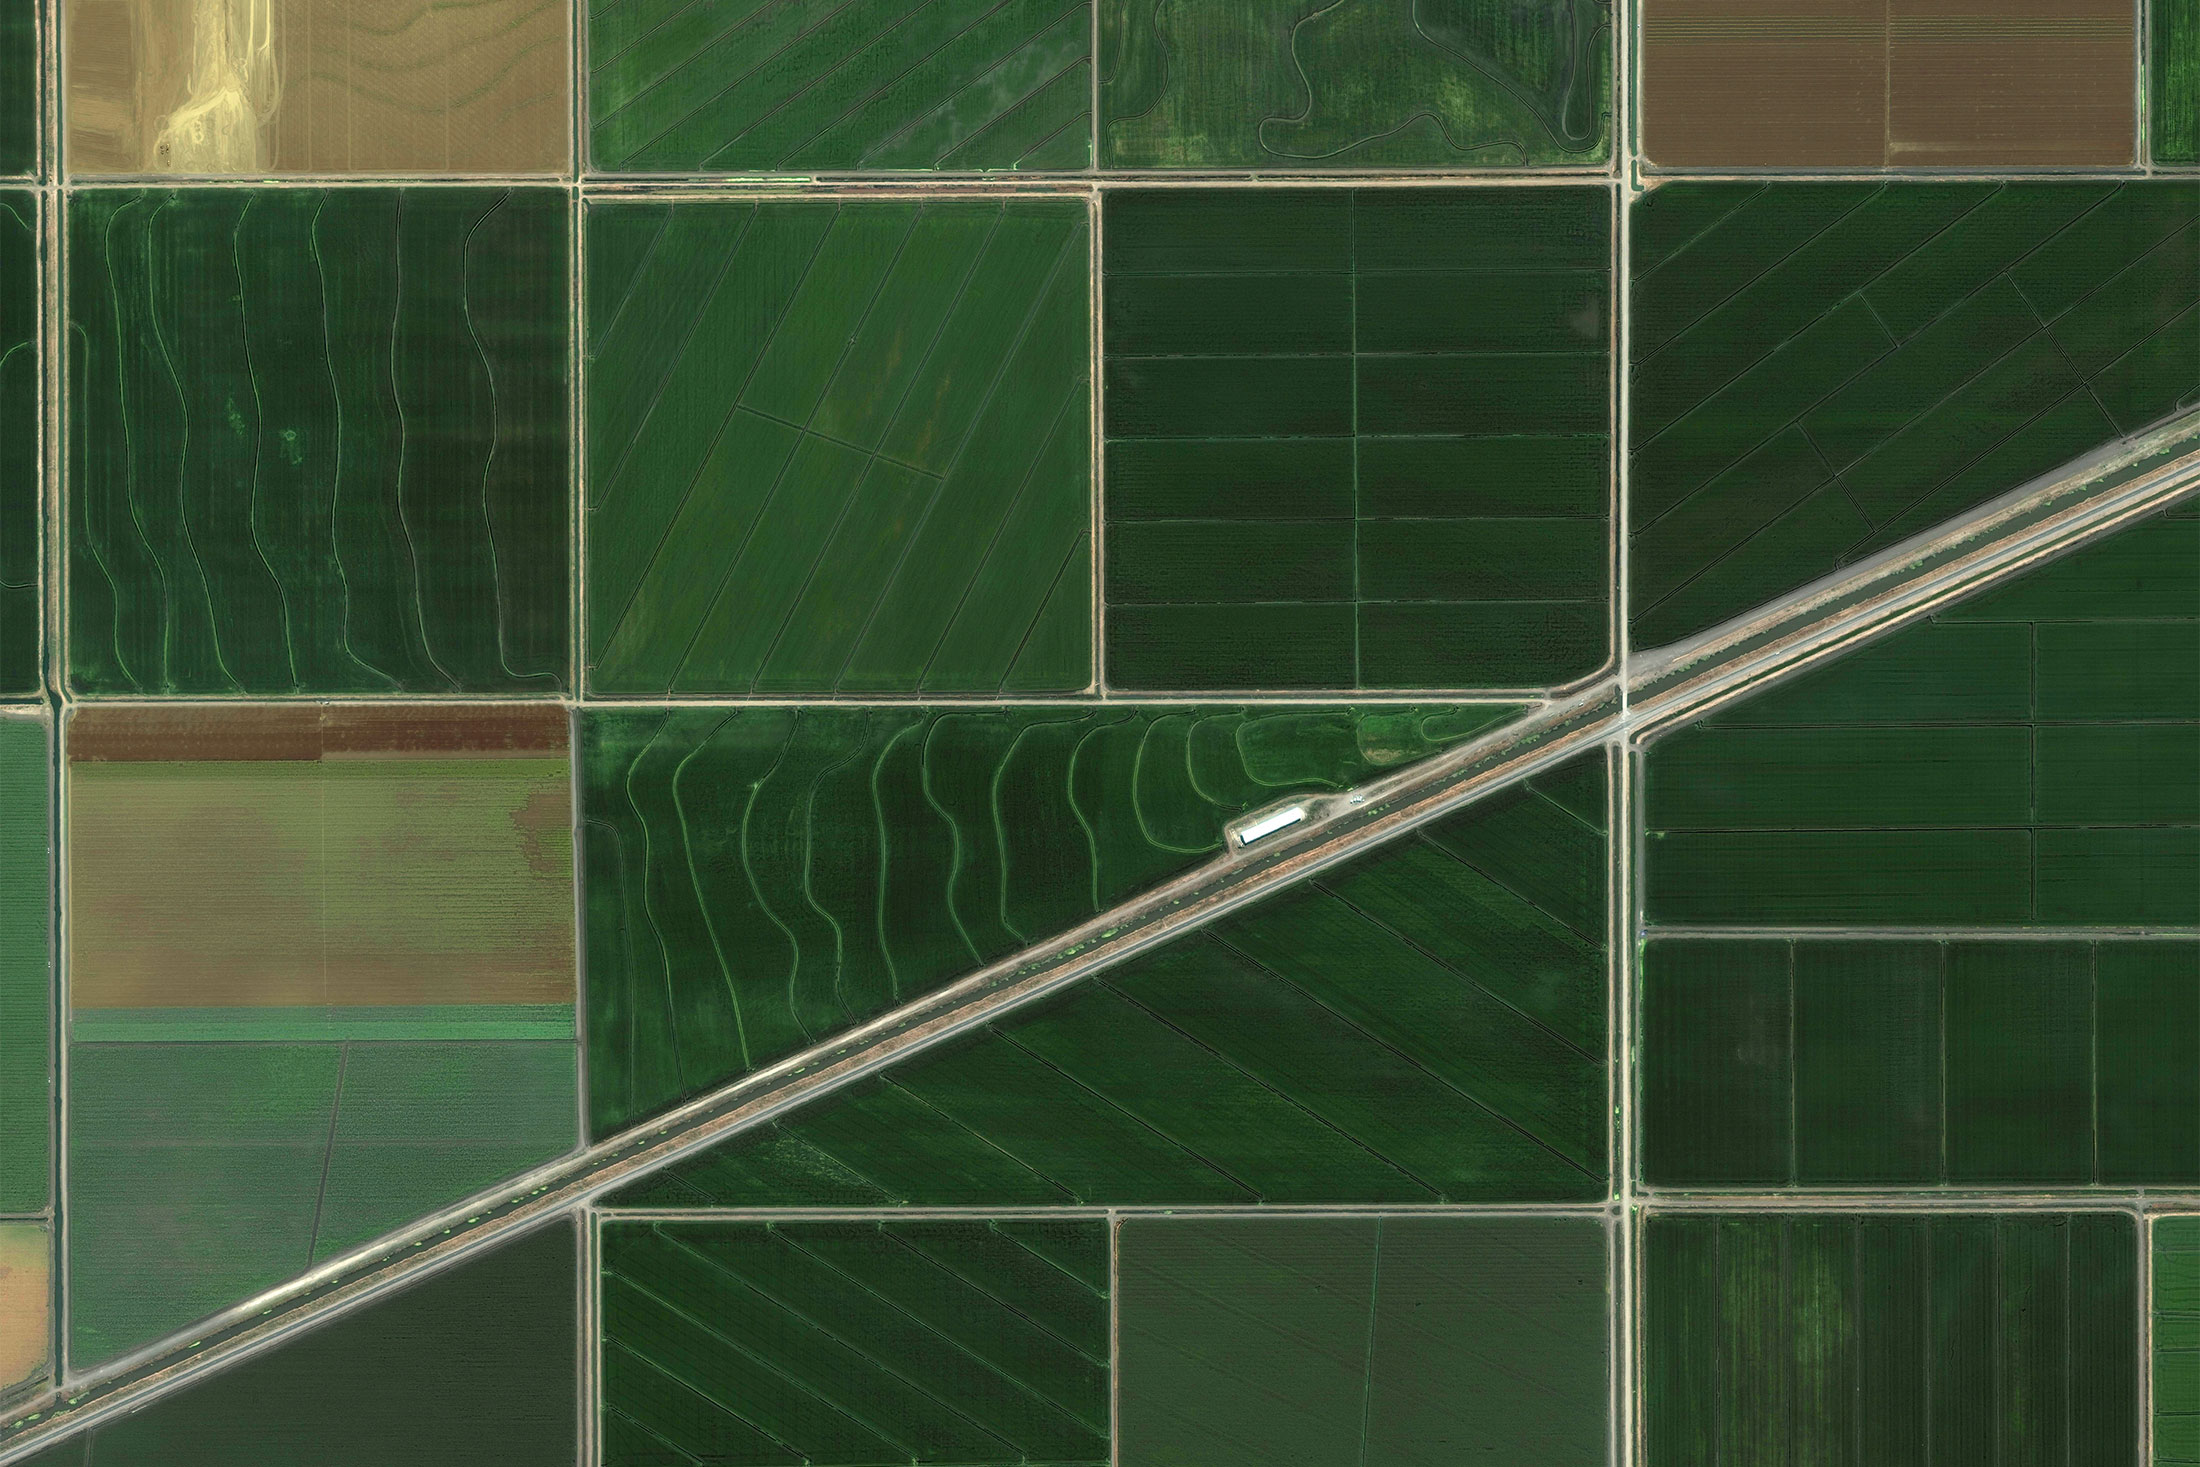
\includegraphics[width=3cm]{../images/illustrations/corn_field.jpeg}
            \end{figure}
         \end{minipage}
         
      \end{itemize}
   \end{itemize}
\end{frame}



%------------------------------------------------------------------------------
\subsection{What is programming}
%------------------------------------------------------------------------------
% ETL
\begin{frame}\frametitle{What is programming}
   \begin{minipage}{0.48\linewidth}

      \begin{itemize}
         \item Software development
         \begin{itemize}
            \item Computer
            \begin{minipage}{0.2\linewidth}
               \begin{figure}[H]
                  
\includegraphics[width=1cm]{../images/illustrations/photoshop.png}
               \end{figure}
            \end{minipage}
            \item Smartphone
            \begin{minipage}{0.2\linewidth}
               \begin{figure}[H]
                  
\includegraphics[width=1cm]{../images/illustrations/instagram.png}
               \end{figure}
            \end{minipage}
            \item Any numerical system
            \begin{minipage}{0.15\linewidth}
               \begin{figure}[H]
                  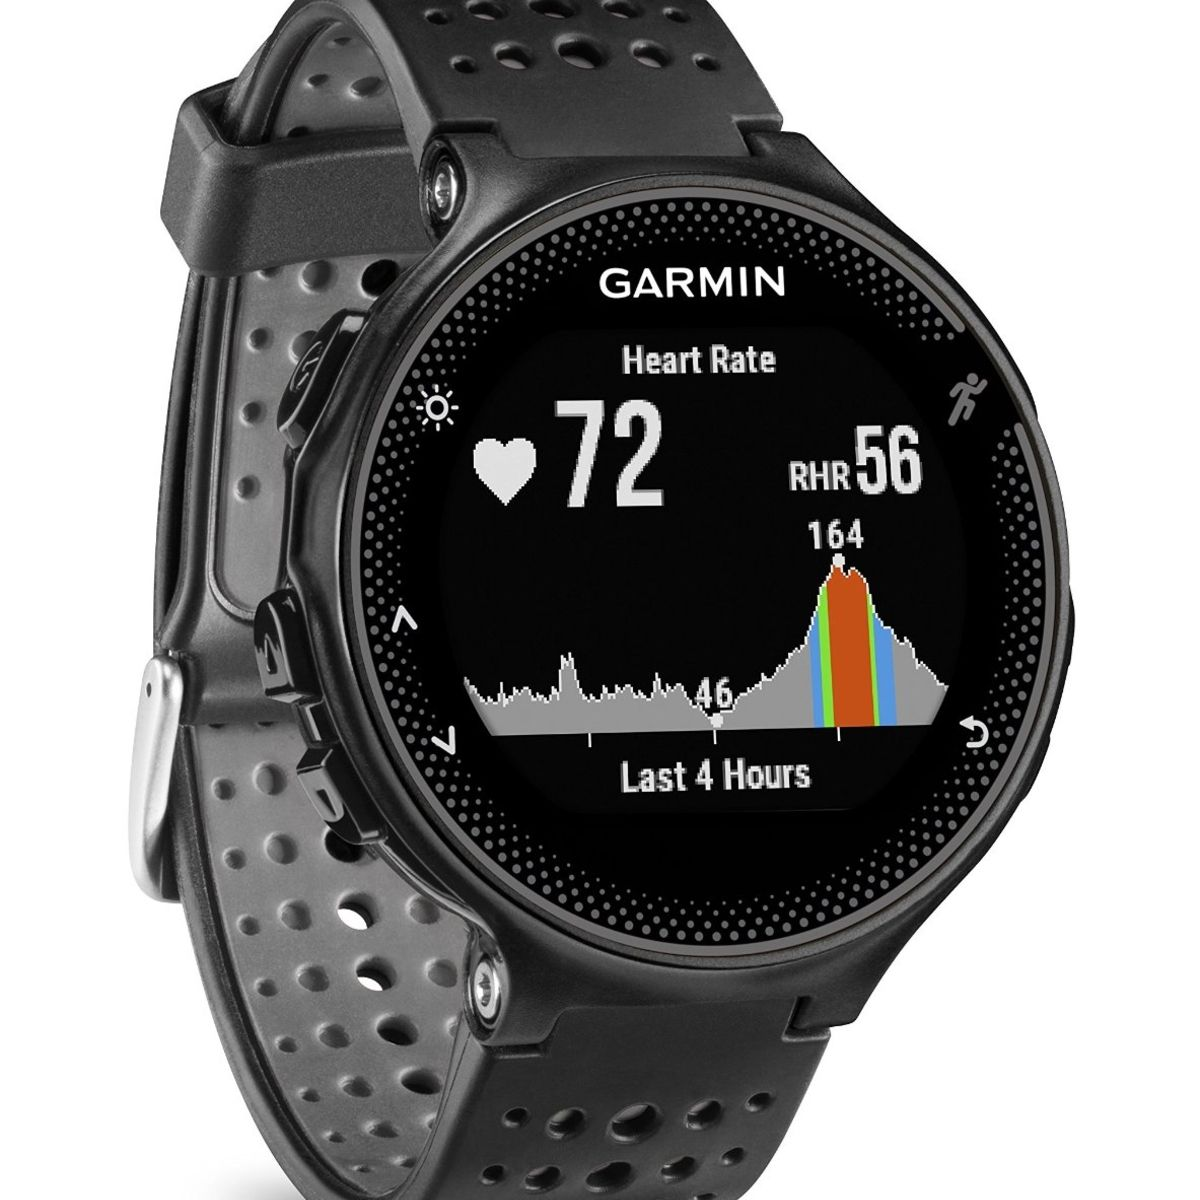
\includegraphics[width=1cm]{../images/illustrations/montre.jpeg}
               \end{figure}
            \end{minipage}
            \hspace{2px}
            \begin{minipage}{0.2\linewidth}
               \begin{figure}[H]
                  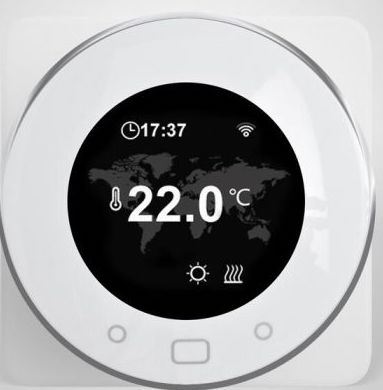
\includegraphics[width=.8cm]{../images/illustrations/chauffage.jpeg}
               \end{figure}
            \end{minipage}
            \begin{minipage}{0.2\linewidth}
               \begin{figure}[H]
                  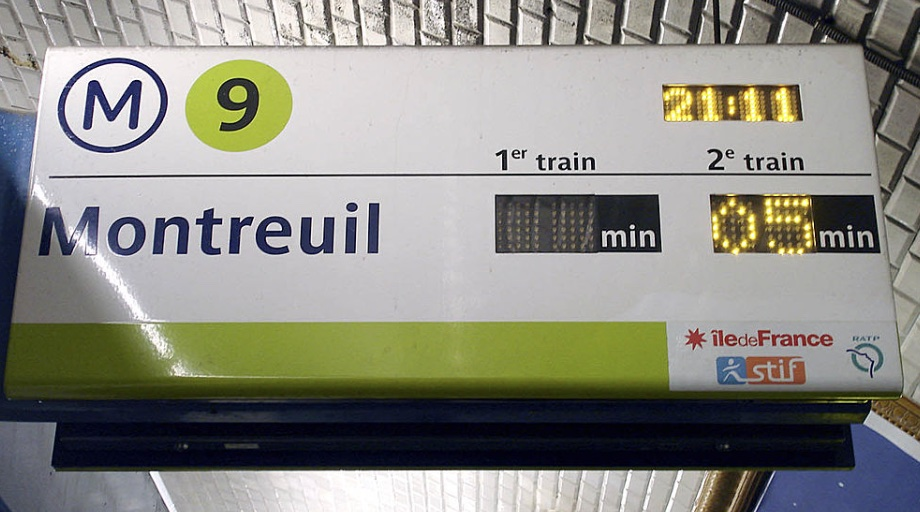
\includegraphics[width=1.5cm]{../images/illustrations/metro.jpg}
               \end{figure}
            \end{minipage}
         \end{itemize}
         \item Automation
         \begin{itemize}
            \item Medium-sized app
            \item Light macro
            \begin{minipage}{0.2\linewidth}
               \begin{figure}[H]
                  
\includegraphics[width=1cm]{../images/illustrations/excel.png}
               \end{figure}
            \end{minipage}
         \end{itemize}
      \end{itemize}
   \end{minipage}
   \begin{minipage}{0.48\linewidth}
      \begin{figure}[H]
         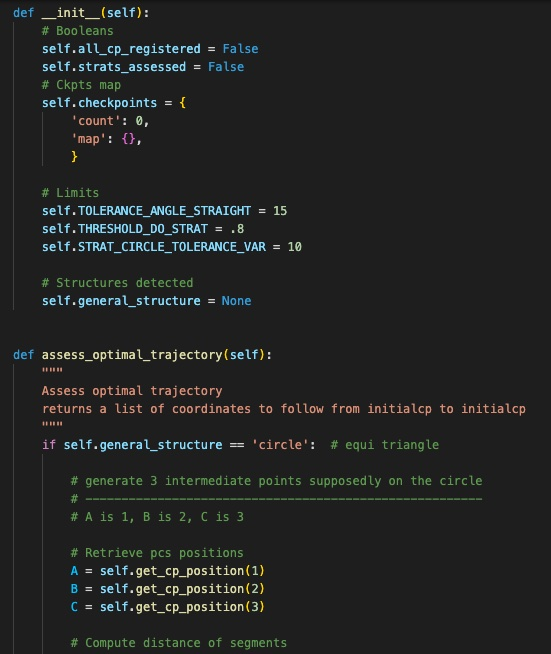
\includegraphics[width=6cm]{../images/illustrations/code.jpg}
      \end{figure}
   \end{minipage}

\end{frame}

\begin{frame}\frametitle{Use cases}
   \begin{itemize}
      \item Data Analysis
      \begin{minipage}{0.2\linewidth}
         \begin{figure}[H]
            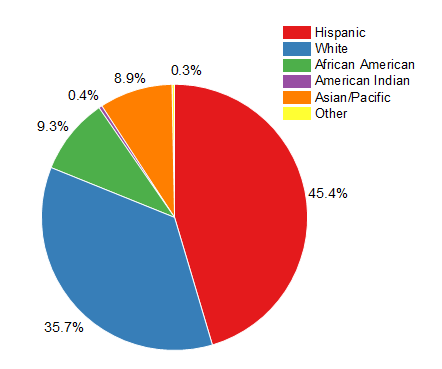
\includegraphics[width=2cm]{../images/illustrations/piechart.png}
         \end{figure}
      \end{minipage}
      \item Python (Dash) visualization app
      \begin{minipage}{0.2\linewidth}
         \begin{figure}[H]
            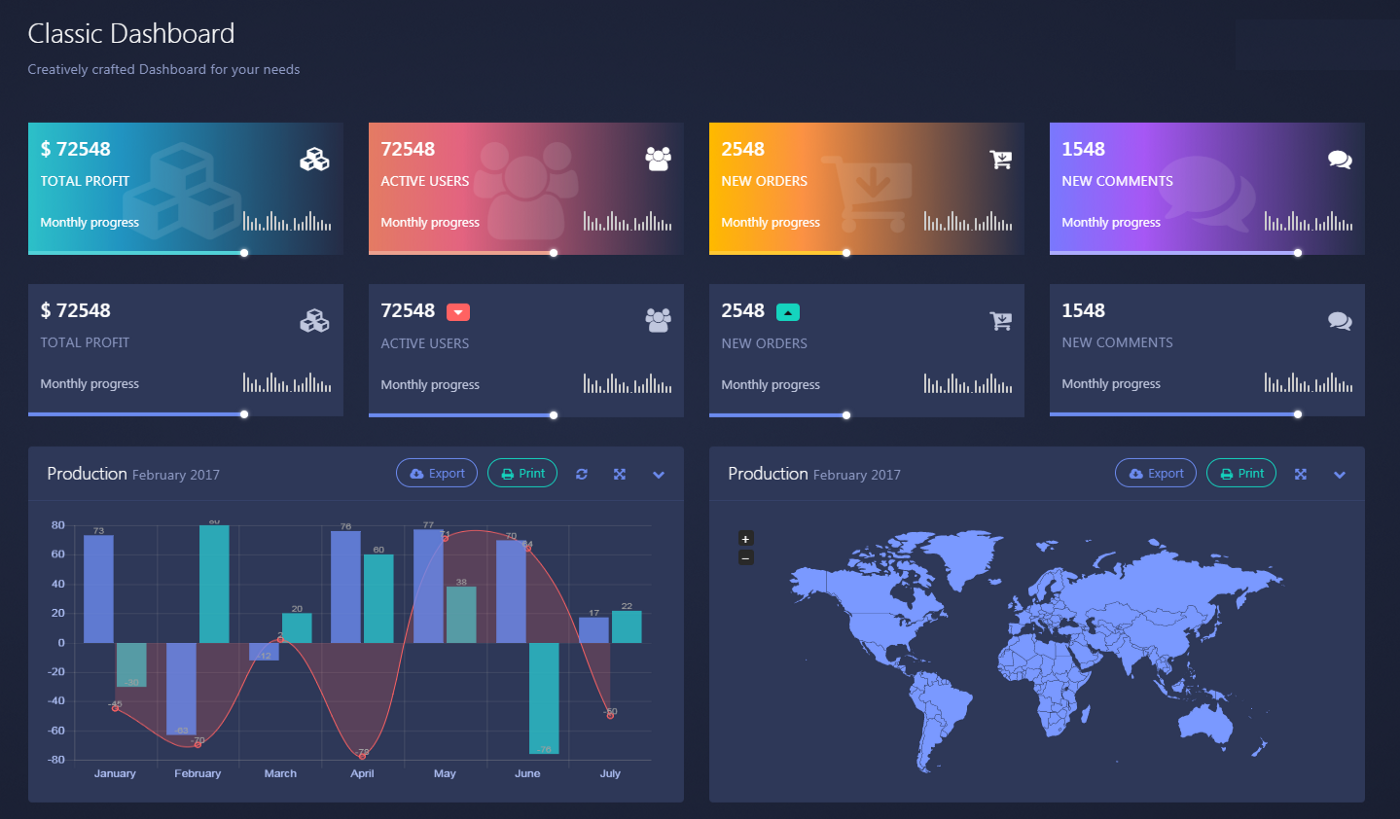
\includegraphics[width=4cm]{../images/illustrations/dashboard.png}
         \end{figure}
      \end{minipage}
      \item VBA macro
      \begin{minipage}{0.2\linewidth}
         \begin{figure}[H]
            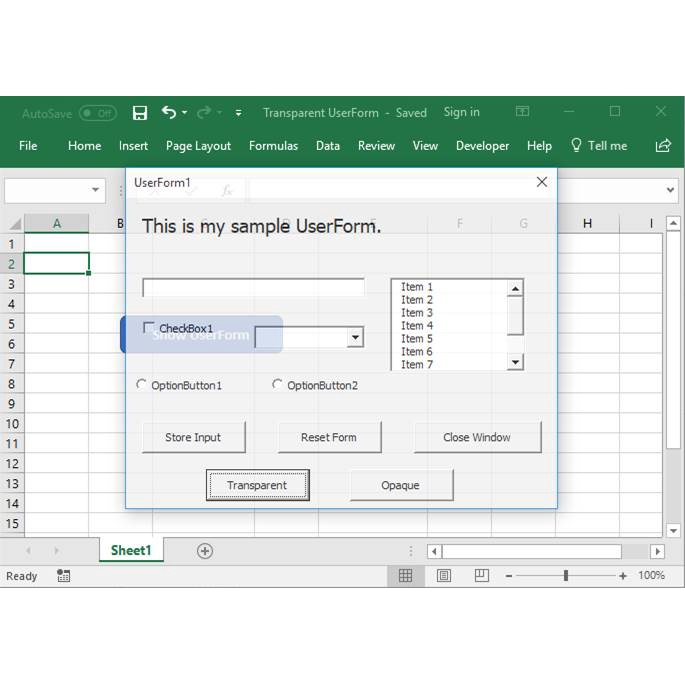
\includegraphics[width=4cm]{../images/illustrations/userform.jpeg}
         \end{figure}
      \end{minipage}
   \end{itemize}
\end{frame}



%------------------------------------------------------------------------------
\subsection{Issues}
%------------------------------------------------------------------------------

\begin{frame}\frametitle{Issues - Lack of robustness in production}
   \begin{itemize}
      \item Poor Model
      \begin{itemize}
         \item Wrong model choice
         \item Overfitted / Underfitted model
         \begin{figure}[H]
            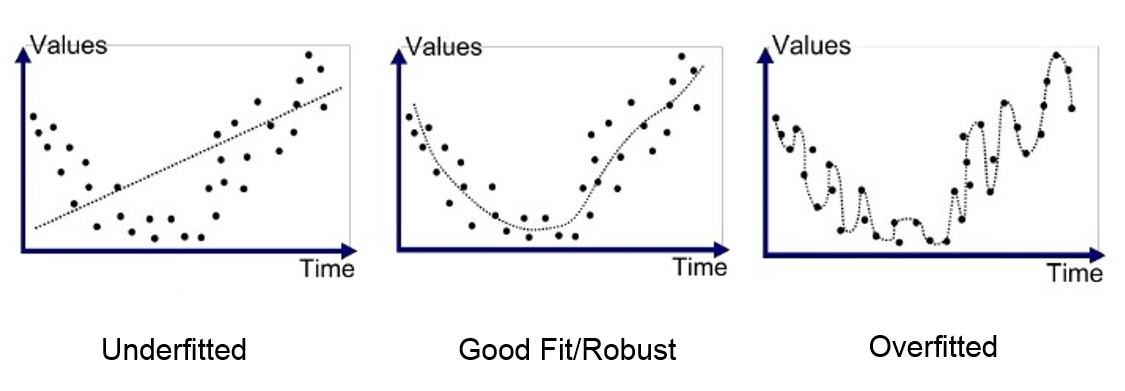
\includegraphics[width=5cm]{../images/illustrations/model_fit.png}
         \end{figure}
      \end{itemize}
      \item Poor data:
      \begin{itemize}
         \item Poor data quality
         \begin{minipage}{0.2\linewidth}
            \begin{figure}[H]
               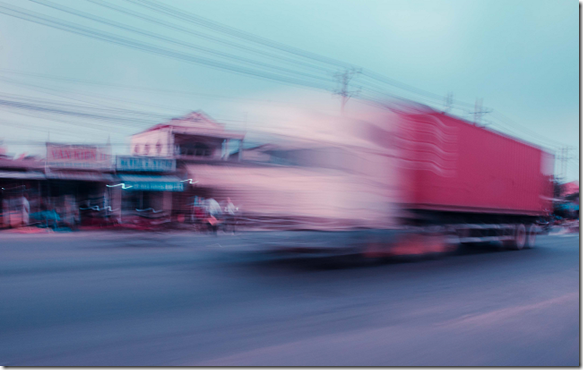
\includegraphics[width=2cm]{../images/illustrations/blurry.png}
            \end{figure}
         \end{minipage}
         \item Data not representative
         \begin{minipage}{0.2\linewidth}
            \begin{figure}[H]
               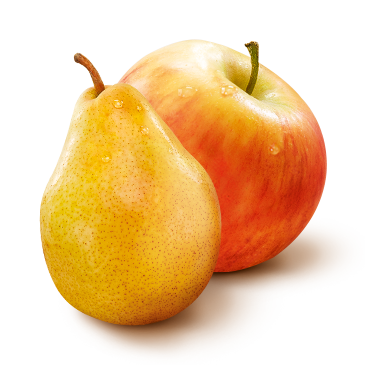
\includegraphics[width=1.5cm]{../images/illustrations/pomme_poire.png}
            \end{figure}
         \end{minipage}
         \item Evolving phenomenom (distribution / covariance shift)
         \begin{minipage}{0.2\linewidth}
            \begin{figure}[H]
               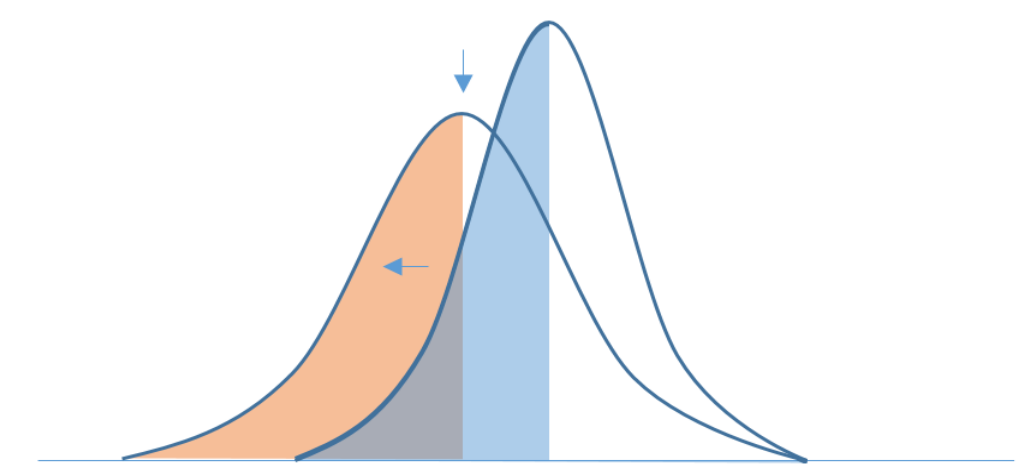
\includegraphics[width=3cm]{../images/illustrations/distribution_shift.png}
            \end{figure}
         \end{minipage}
      \end{itemize}
   \end{itemize}   
\end{frame}

\begin{frame}\frametitle{Issues - Attacks}
   % TODO: add references articles to US models used for determining justice decisions
   \begin{itemize}
      \item Adversarial attack: Pixel wise, noise, post it
      \begin{minipage}{0.4\linewidth}
         \begin{figure}[H]
            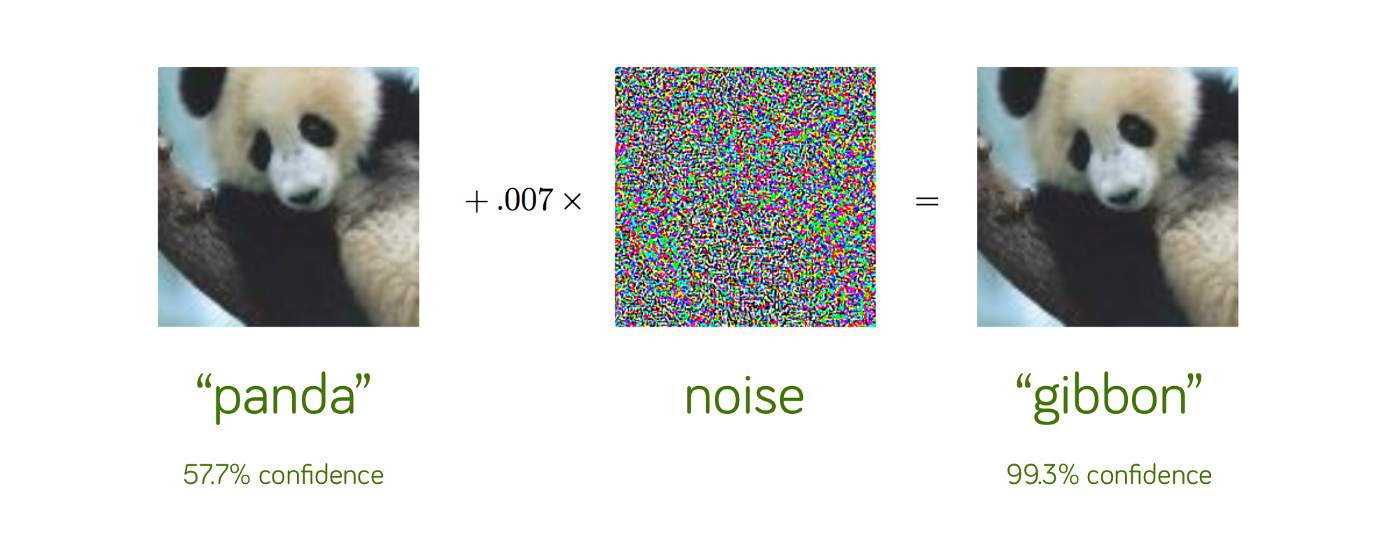
\includegraphics[width=6cm]{../images/illustrations/adversarial_attack.png}
         \end{figure}
      \end{minipage}
      \item Modify model weights value (require access to the model)
      \item Poison attack: provide bad examples for continuous training
   \end{itemize}
\end{frame}

\begin{frame}\frametitle{Issues - Ethics (bias reproduction)}
   \begin{itemize}
      \item Racism\footnote{\href{https://www.kdnuggets.com/2021/06/ethics-fairness-ai.html}{Racism in AI}}, sexism
      \hspace{20px}
      \begin{minipage}{0.2\linewidth}
         \begin{figure}[H]
            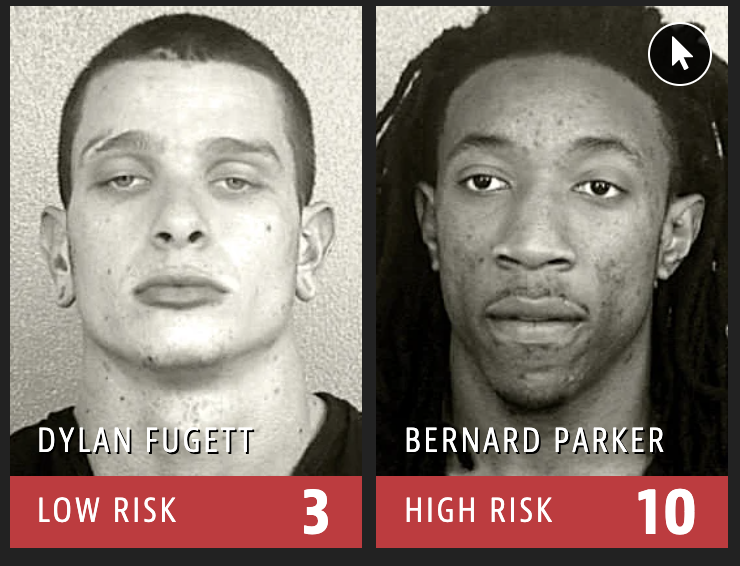
\includegraphics[width=3cm]{../images/illustrations/racism.png}
         \end{figure}
      \end{minipage}

      \item Any discrimination
      \begin{itemize}
         \item Health history
         \item Carrier history
         \item Any mater on which humans have bias
      \end{itemize}
   \end{itemize}
\end{frame}

\begin{frame}\frametitle{Issues - RGPD}

   \begin{minipage}{0.38\linewidth}
      \begin{itemize}
         \item Personal data
         \begin{itemize}
            \item Passwords
            \item Ethnicity
            \item Salary
            \item Health issues
         \end{itemize}
      \end{itemize}t
   \end{minipage}
   \begin{minipage}{0.6\linewidth}
      \begin{figure}[H]
         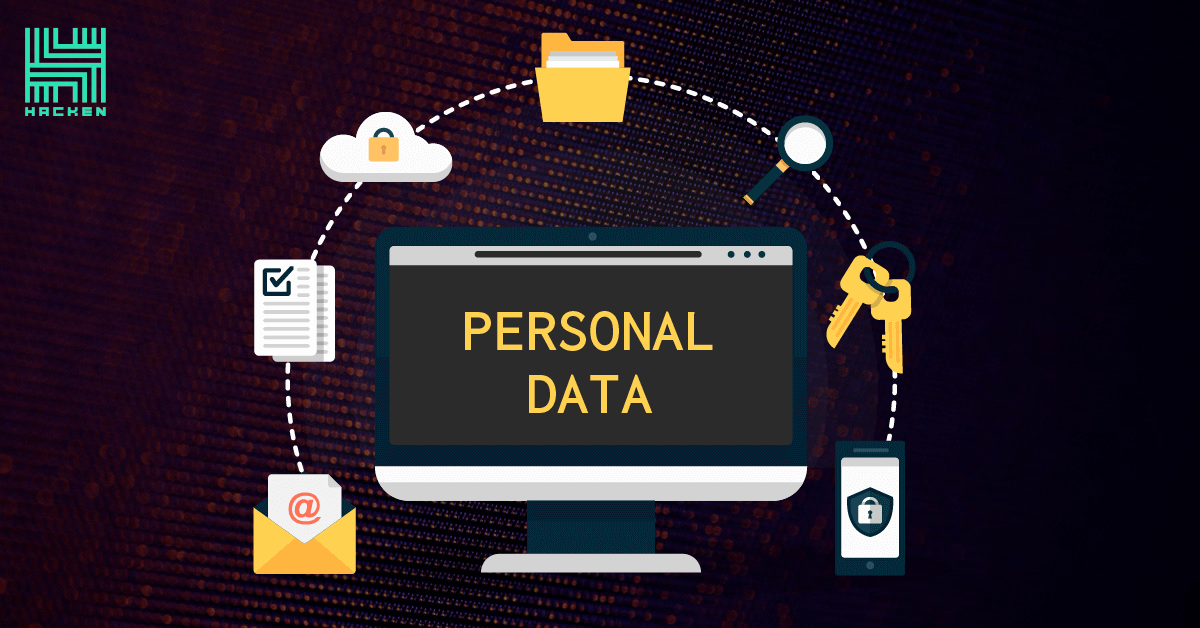
\includegraphics[width=6cm]{../images/illustrations/personal_data.png}
      \end{figure}
   \end{minipage}
\end{frame}



%------------------------------------------------------------------------------
\subsection{Resources}
%------------------------------------------------------------------------------
\begin{frame}\frametitle{Resources}
   \begin{itemize}
      \item Stack Overflow \hspace{3px}
      \begin{minipage}{0.4\linewidth}
         \begin{figure}[H]
            
\includegraphics[width=2.5cm]{../images/illustrations/stackoverflow.png}
         \end{figure}
      \end{minipage}
   
      \item Towards Data Science
      \begin{minipage}{0.3\linewidth}
         \begin{figure}[H]
            
\includegraphics[width=1.5cm]{../images/illustrations/tds.png}
         \end{figure}
      \end{minipage}
      \item Blogs of AI research Labs (GAFAM, OpenAI)
      \item Research Papers
      \begin{itemize}
         \item Google Scholar
         \item Arxiv
         \item Papers with code
         \begin{minipage}{0.3\linewidth}
            \begin{figure}[H]
               
\includegraphics[width=2.5cm]{../images/illustrations/papers_with_code.png}
            \end{figure}
         \end{minipage}

      \end{itemize}
   \end{itemize}
\end{frame}


\end{document}
